%%%%%%%%%%%%%%%%%%%%%%%%%
% Dokumentinformationen %
%%%%%%%%%%%%%%%%%%%%%%%%%
\newcommand{\titleinfo}{Integraltransformationen - Formelsammlung}
\newcommand{\authorinfo}{Braun \& Co, J\"urg \& Co, Hannes Revision}
\newcommand{\versioninfo}{$Revision: 2 $ - powered by \LaTeX}

%%%%%%%%%%%%%%%%%%%%%%%%%%%%%%%%%%%%%%%%%%%%%
% Standard projektübergreifender Header für
% - Makros 
% - Farben
% - Mathematische Operatoren
%
% DORT NUR ERGÄNZEN, NICHTS LÖSCHEN
%%%%%%%%%%%%%%%%%%%%%%%%%%%%%%%%%%%%%%%%%%%%%

% Genereller Header
\documentclass[10pt,twoside,a4paper,fleqn]{article}
% Dateiencoding
\usepackage[utf8]{inputenc}
% Seitenränder
\usepackage[left=1cm,right=1cm,top=1cm,bottom=1cm,includeheadfoot]{geometry}
% Sprachpaket
\usepackage[ngerman]{babel,varioref}

% Pakete
\usepackage{amssymb,amsmath,fancybox,graphicx,lastpage,wrapfig,fancyhdr,hyperref,verbatim,floatflt,multicol,multirow,rotating,pdflscape,array,longtable,listings}

% Zum Bilder einfach in Tabellen einfügen (valign=t)
\usepackage[export]{adjustbox}

%%%%%%%%%%%%%%%%%%%%
% Generelle Makros %
%%%%%%%%%%%%%%%%%%%%
\newcommand{\skript}[1]{$_{\textcolor{red}{\mbox{\small{Skript S.#1}}}}$}
\newcommand{\verweis}[2]{\small{(siehe auch \ref{#1}, #2 (S. \pageref{#1}))}}
\newcommand{\verweiskurz}[1]{(\small{siehe \ref{#1}\normalsize)}}
\newcommand{\subsubadd}[1]{\textcolor{black}{\mbox{#1}}}
\newcommand{\formelbuch}[1]{$_{\textcolor{red}{\mbox{\small{S#1}}}}$}

\newcommand{\kuchling}[1]{$_{\textcolor{red}{\mbox{\small{Kuchling #1}}}}$}
\newcommand{\stoecker}[1]{$_{\textcolor{orange}{\mbox{\small{Stöcker #1}}}}$}
\newcommand{\sachs}[1]{$_{\textcolor{blue}{\mbox{\small{Sachs S. #1}}}}$}
\newcommand{\hartl}[1]{$_{\textcolor{green}{\mbox{\small{Hartl S. #1}}}}$}

\newcommand{\schaum}[1]{\tiny Schaum S. #1}

\newcommand{\skriptsection}[2]{\section{#1 {\tiny Skript S. #2}}}
\newcommand{\skriptsubsection}[2]{\subsection{#1 {\tiny Skript S. #2}}}
\newcommand{\skriptsubsubsection}[2]{\subsubsection{#1 {\tiny Skript S. #2}}}

\newcommand{\matlab}[1]{\footnotesize{(Matlab: \texttt{#1})}\normalsize{}}

%%%%%%%%%%
% Farben %
%%%%%%%%%%
\usepackage{xcolor}

%%%%%%%%%%%%%%%%%%%%%%%%%%%%
% Mathematische Operatoren %
%%%%%%%%%%%%%%%%%%%%%%%%%%%%
\DeclareMathOperator{\sinc}{sinc}
\DeclareMathOperator{\sgn}{sgn}
\DeclareMathOperator{\Real}{Re}
\DeclareMathOperator{\Imag}{Im}
%\DeclareMathOperator{\e}{e}
\DeclareMathOperator{\cov}{cov}
\DeclareMathOperator{\PolyGrad}{PolyGrad}

%Makro für 'd' von Integral- und Differentialgleichungen 
\newcommand*{\diff}{\mathop{}\!\mathrm{d}}


%%%%%%%%%%%%%%%%%%%%%%%%%%%
% Fouriertransformationen %
%%%%%%%%%%%%%%%%%%%%%%%%%%%
\usepackage{trfsigns, trsym}
%\unitlength1cm
% Zeitbereich -- Frequenzbereich
%\newcommand{\laplace}
%{
%\begin{picture}(1,0.5)
%\put(0.2,0.1){\circle{0.14}}\put(0.27,0.1){\line(1,0){0.5}}\put(0.77,0.1){\circle*{0.14}}
%\end{picture}
%}
% Frequenzbereich -- Zeitbereich
%\newcommand{\Laplace}
%{
%\begin{picture}(1,0.5)
%\put(0.2,0.1){\circle*{0.14}}\put(0.27,0.1){\line(1,0){0.45}}\put(0.77,0.1){\circle{0.14}}
%\end{picture}
%}


% Fouriertransformationen
\unitlength1cm
\newcommand{\FT}
{
\begin{picture}(1,0.5)
\put(0.2,0.1){\circle{0.14}}\put(0.27,0.1){\line(1,0){0.5}}\put(0.77,0.1){\circle*{0.14}}
\end{picture}
}


\newcommand{\IFT}
{
\begin{picture}(1,0.5)
\put(0.2,0.1){\circle*{0.14}}\put(0.27,0.1){\line(1,0){0.45}}\put(0.77,0.1){\circle{0.14}}
\end{picture}
}




%%%%%%%%%%%%%%%%%%%%%%%%%%%%
% Allgemeine Einstellungen %
%%%%%%%%%%%%%%%%%%%%%%%%%%%%
%PDF Info
\hypersetup{pdfauthor={\authorinfo},pdftitle={\titleinfo},colorlinks=false}
\author{\authorinfo}
\title{\titleinfo}

%%%%%%%%%%%%%%%%%%%%%%%
% Kopf- und Fusszeile %
%%%%%%%%%%%%%%%%%%%%%%%
\pagestyle{fancy}
\fancyhf{}
%Linien oben und unten
\renewcommand{\headrulewidth}{0.5pt} 
\renewcommand{\footrulewidth}{0.5pt}

\fancyhead[L]{\titleinfo{ }\tiny{(\versioninfo)}}
%Kopfzeile rechts bzw. aussen
\fancyhead[R]{Seite \thepage { }von \pageref{LastPage}}
%Fusszeile links bzw. innen
\fancyfoot[L]{\footnotesize{\authorinfo}}
%Fusszeile rechts bzw. ausen
\fancyfoot[R]{\footnotesize{\today}}
%Lizenz CC-BY-NC-SA
% Headerfile für die Einbindung einer Lizenzgrafik in den Footer
% Verwendung: \lizenz{cc-by-nc-sa}{small}
\newcommand{\lizenz}[2]
{
\fancyfoot[C]{
  \includegraphics[width=1.6cm]{./header/lizenzen/#1/#2.png}
}
}
\lizenz{cc-by-nc-sa}{small}
%Einrücken verhindern versuchen
\setlength{\parindent}{0pt}

% Zeilenhöhe Tabellen:
\newcommand{\arraystretchOriginal}{1.5}
\renewcommand{\arraystretch}{\arraystretchOriginal}


\usepackage{tikz}

% Möglichst keine Ergänzungen hier, sondern in header.tex
\begin{document}
%%%%%%%%%%%%%%%%%%%%%%%%%%%%%%%%%%%%%%%%%%%%%%%%%%%%%%%%%%%%%%%%%%%%%%%%%%%%%%%%%%%%%%%%%%%%%%%%
%%%%%%%%%%%%%%%%%%%%%%%%%%%%%%%%%%%%%%%%%%%%%%%%%%%%%%%%%%%%%%%%%%%%%%%%%%%%%%%%%%%%%%%%%%%%%%%%

% Einleitung

\section{Varianten der Integraltransformationen}
\begin{tabular}{|l||l|l|}
\hline
\textbf{Signalart}
	& diskret
	& kontinuierlich \\
\hline \hline
periodisch
	& Diskrete Fourier-Transformation
	& Fourierreihe \\
\hline
impulsförmig
	& ``Fourierreihe mit $T = Impulsdauer$''
	& Fourierintegral \\
\hline
kausal
	& Z-Transformation
	& Laplace-Transformation \\
\hline
\end{tabular}

% Signale und Systeme
\section{Signale und Systeme}
	\begin{tabular}{|l|l|}
    	\hline
    	\textbf{Linearität} & \textbf{Zeitinvarianz}\\
    	\hline
    	$S(x1+x2)=S(x1)+S(x2)$ & $S(x(t-t_0)=S(x)\cdot x(t-t_0)$ \\
    	$S(c\cdot x)=c\cdot S(x)$ & \\
		\hline    
    \end{tabular}
  	
	\subsection{Lineare Systeme}
		\textbf{Basissignale}
		\begin{list}{$\bullet$}{\setlength{\itemsep}{0cm} \setlength{\parsep}{0cm} \setlength{\topsep}{0cm}} 
          \item Lineare Systeme sind durch die Antworten auf die
          Basissignale bestimmt.
          \item Basissignale müssen linear unabhängig voneinander sein, d.h. ein
		Basissignal darf nicht durch \textbf{Linearkombination} anderer Basissignale
		darstellbar sein          
		  \item Alle möglichen Eingangs-Funktionen müssen durch eine Linearkombination der
		Basissignale dargestellt werden können. $\Rightarrow$ \textbf{Periode des Eingangssignals =	Anzahl Basissignale}
        \end{list}
        \vspace{.2cm}
		\textbf{Berechnung der Systemantwort aufgrund der Basissignale und der
		Anregung}\\
		1. Eingangssignal $x$ als Linearkombination der Basisvektoren darstellen
		$\Rightarrow$ lineares Gleichungssystem\\
		$\Rightarrow x=r\cdot a + s\cdot b + t\cdot c\qquad$ ($x=$
		Eingangssignal; $a,b,c=$ Basisvektoren; $r,s,t=$
		Linearkombinationsparameter)\\ 
		2. Systemantwort $y=r\cdot S(a) + s\cdot S(b) + t\cdot S(c); \qquad (S(a)=$
		Systemantwort der Basis $a$)
	
	\subsection{Lineare zeitinvariante Systeme (LTI-Systeme)}
		LTI-Systeme sind durch ihre Impulsantwort $h$ vollständig bestimmt\\ \\
		\textbf{Berechnung der Systemantwort von diskreten LTI-Systemen}\\
		$\; y=x*h \qquad$ ($y=$ Systemantwort; $x=$ Eingangssignal; $h=$
		Impulsantwort)\\
		
		\textbf{Berechnung der Systemantwort von kontinuierlichen LTI-Systemen}\\
		\begin{tabular}{ll}
			\parbox{8cm}{
			$$s_2(t) = h(t) * s_1(t) \laplace S_2(s) = H(s) S_1(s)$$
			$$h(t) \laplace H(s)$$}
			& \parbox{4cm}{
			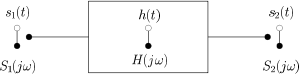
\includegraphics[width=5cm]{./bilder/utf-theorie.png}}\\
		\end{tabular}	
		
	\subsection{Faltung}
	$y(t) = f(t)\ast g(t) = g(t) \ast f(t) = (f \ast g)(t) :=
	\int\limits_{-\infty}^\infty f(u) \cdot g(t-u)\,du =
	\int\limits_{-\infty}^\infty f(t-u) \cdot h(u)\,du $ \\
	wobei gilt: $h\left/t\right) g(t) = $ Impulsantwort des Systems \\
	Hat $g\left(t\right)$ keine negative Argumente dann gilt :
	$\left(g \ast f \right)\left(t\right)=\int\limits_{-\infty}^t f(u) \cdot
	g(t-u)\,du$\\
	Hat $f\left(t\right)$ keine negative Argumente (Einschaltvorgang) dann gilt :
	$\left(g \ast f \right)\left(t\right)=\int\limits_{0}^t f(u) \cdot
	g(t-u)\,du$\\
	Bei einer Faltung mit einer $\delta\left(t\right)$Funktion
	gilt:$f\left(t\right) \ast \delta\left(t\right) = f\left(t\right)$\\
	
	\newpage
	
	\begin{multicols}{2}
		\textbf{grafische Interpretation:}
		\begin{enumerate}
  			\item einfacheres Signal an der Y-Achse spiegeln
  			\item Verschiebung um t nach rechts
  			\item Multiplikation und Integration der beiden Signale
		\end{enumerate}
		\columnbreak
		\textbf{Bestimmung der Grenzen:}
		\begin{enumerate}
		  \item Koordinatensystem: X-Achse: t, Y-Achse: u
		  \item Erster Faktor $\rightarrow$ Streifen parallel zur X-Achse
		  \item Zweiter Faktor $\rightarrow$ Streiffen parallel zur $45^{\circ}$-Geraden
		  \item Grenzen für ein bestimmtes t ablesen
		\end{enumerate}
	\end{multicols}	



% Diskrete Fourier Transformation
%\section{Diskrete Fourier Transformation (DFT)}
	$$\boxed{s(h)=\sum_{k=0}^{N-1}\hat c_k e^{jhk\frac{2\pi}{N}}=\sum_{k=0}^{N-1}
	\left[ \hat{a}_k \cos\left(hk \frac{2 \pi}{N}\right)+\hat{b}_k \sin\left(hk
	\frac{2 \pi}{N}\right) \right]} \qquad N=\text{Periodenanzahl}$$\\
	$$\hat{c}_k=\frac{1}{N}\sum_{h=0}^{N-1}s(h)
	e^{-jhk\frac{2\pi}{N}}=\hat{a}_k-j\hat{b}_k \qquad \hat{a}_k=\frac{1}{N}
	\sum_{h=0}^{N-1}s(h) \cos\left(hk \frac{2 \pi}{N}\right)=Re(\hat{c}_k) \qquad
	\hat{b}_k=\frac{1}{N} \sum_{h=0}^{N-1}s(h) \sin\left(hk \frac{2
	\pi}{N}\right)=-Im(\hat{c}_k)$$\\	

	\subsection{Berechnung mit Matrizen}
		\textbf{Transformation}\\
		1. Periode $N$ des Signalvektors $\vec{s}=
		\begin{bmatrix}
		s(0) \\
		s(1) \\
		s(N-1)\\
		\end{bmatrix}$ bestimmen\\ \\
		2. Einheitswurzel $w$ berechnen: $w=e^{j\frac{2 \pi}{N}}$\\ \\
		3. Matrix $W$ berechnen: $W=
		\begin{bmatrix}
		w^0 & w^0 & w^0 & \ldots & w^0\\
		w^0 & w^1 & w^2 & \ldots & w^{N-1}\\
		w^0 & w^2 & w^4 & \ldots & w^{2(N-1)}\\
		\ldots & \ldots & \ldots & \ldots & \ldots\\
		w^0 & w^{N-1} & w^{2(N-1)} & \ldots & w^{(N-1)(N-1)}                        
		\end{bmatrix}$\\ \\
		4. Matrix $V$ berechnen: $V=W^*$ (konj. komplex)\\ \\
		5. Koeffizienten bzw. Fouriertransformierte $\vec{c}$ berechnen:
		$\vec{c}=\frac{1}{N}V\vec{s}$\\

		\begin{minipage}{13cm}
			\textbf{Rücktransformation}\\
			1. Matrix $W$ (wie bei der Transformation beschrieben) berechnen \\
			2. Signalvektor $\vec{s}$ berechnen: $\vec{s}=W\vec{c}$	
			\subsection{Matrizenmultiplikation}
			\begin{tabular}{ll}
				$\frac14
				\begin{bmatrix}
				    6 & -1 & 4 \\
				    3 & 2 & -2 \\
				    0 & -3 & -1
				\end{bmatrix}
				\cdot
				\begin{bmatrix}
					1 \\
				    4 \\
				    3 
				\end{bmatrix}
				=
				\frac14
				\begin{bmatrix}
					6 \cdot 1 + (-1) \cdot 4 + 4 \cdot 3\\
					3 \cdot 1 + 2 \cdot  4 + (-2) \cdot 3\\
					0 \cdot 1 + (-3) \cdot 4 + (-1) \cdot 3  
				\end{bmatrix}
				=
				\frac14
				\begin{bmatrix}
				    14\\
				    5\\
				    -15
				\end{bmatrix}
				=
				\begin{bmatrix}
		        	3.5\\
		        	1.25\\
		        	-3.75
		        \end{bmatrix}$
		    \end{tabular}		
        \end{minipage}
		\begin{minipage}[c]{5cm}
        	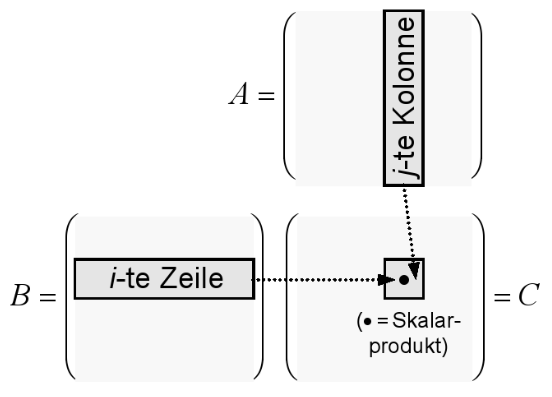
\includegraphics[width=5cm]{./bilder/matrix.png}
        \end{minipage}
		
	\subsection{Einige W-Matrizen}
		\begin{tabular}{l l l l}
        N = 2 & N = 3 & N = 4 & N = 6\\
		$\begin{bmatrix}
		1 & 1\\
		1 & -1\\              
		\end{bmatrix}$ &
		$\begin{bmatrix}
		1 & 1 & 1\\
		1 & -\frac{1}{2}+j\frac{\sqrt{3}}{2} & -\frac{1}{2}-j\frac{\sqrt{3}}{2}\\
		1 & -\frac{1}{2}-j\frac{\sqrt{3}}{2} & -\frac{1}{2}+j\frac{\sqrt{3}}{2}\\
		\end{bmatrix}$ &
		$\begin{bmatrix}
		1 & 1 & 1 & 1 \\
		1 & j & -1 & -j\\
		1 & -1 & 1 & -1\\
		1 & -j & -1 & j\\                   
		\end{bmatrix}$ &
		$\begin{bmatrix}
		1 & 1 & 1 & 1 & 1 & 1\\
		1 & \frac{1}{2}+j\frac{\sqrt{3}}{2} & -\frac{1}{2}+j\frac{\sqrt{3}}{2} & -1
		& -\frac{1}{2}-j\frac{\sqrt{3}}{2} & \frac{1}{2}-j\frac{\sqrt{3}}{2}\\
		1 & -\frac{1}{2}+j\frac{\sqrt{3}}{2} & -\frac{1}{2}-j\frac{\sqrt{3}}{2} & 1
		& -\frac{1}{2}+j\frac{\sqrt{3}}{2} & -\frac{1}{2}-j\frac{\sqrt{3}}{2}\\
		1 & -1 & 1 & -1 & 1 & -1\\
		1 & -\frac{1}{2}-j\frac{\sqrt{3}}{2} & -\frac{1}{2}+j\frac{\sqrt{3}}{2} & 1
		& -\frac{1}{2}-j\frac{\sqrt{3}}{2} & -\frac{1}{2}+j\frac{\sqrt{3}}{2}\\ 
		1 & \frac{1}{2}-j\frac{\sqrt{3}}{2} & -\frac{1}{2}-j\frac{\sqrt{3}}{2} & -1
		& -\frac{1}{2}+j\frac{\sqrt{3}}{2} & \frac{1}{2}+j\frac{\sqrt{3}}{2}\\ 
		\end{bmatrix}$
		\end{tabular}

		\begin{tabular}{l }
        N = 8\\
 		$\begin{bmatrix}
		1 & 1 & 1 & 1 & 1 & 1 & 1 & 1\\ 
		1 & \frac{\sqrt{2}}{2}+\frac{\sqrt{2}}{2}j & j &
		-\frac{\sqrt{2}}{2}+\frac{\sqrt{2}}{2}j & -1 & 
		-\frac{\sqrt{2}}{2}-\frac{\sqrt{2}}{2}j & -j & 
		\frac{\sqrt{2}}{2}-\frac{\sqrt{2}}{2}j\\
		1 & j & -1 & -j & 1 & j & -1 & -j\\
		1 &	-\frac{\sqrt{2}}{2}+\frac{\sqrt{2}}{2}j & -j & 
		\frac{\sqrt{2}}{2}+\frac{\sqrt{2}}{2}j & -1 & 
		\frac{\sqrt{2}}{2}-\frac{\sqrt{2}}{2}j & j &
		-\frac{\sqrt{2}}{2}-\frac{\sqrt{2}}{2}j\\
		1 & -1 & 1 & -1 & 1 & -1 & 1 & -1\\
		1 &	-\frac{\sqrt{2}}{2}-\frac{\sqrt{2}}{2}j & j &
		\frac{\sqrt{2}}{2}-\frac{\sqrt{2}}{2}j & -1 &
		\frac{\sqrt{2}}{2}+\frac{\sqrt{2}}{2}j & -j &
		-\frac{\sqrt{2}}{2}+\frac{\sqrt{2}}{2}j\\
		1 & -j & -1 & j & 1 & -j & -1 & j\\
		1 &	\frac{\sqrt{2}}{2}-\frac{\sqrt{2}}{2}j & -j & 
		-\frac{\sqrt{2}}{2}-\frac{\sqrt{2}}{2}j & -1 &
		-\frac{\sqrt{2}}{2}+\frac{\sqrt{2}}{2}j & j &
		\frac{\sqrt{2}}{2}+\frac{\sqrt{2}}{2}j
		\end{bmatrix}$
		\end{tabular}


	
	
	
	
%\newpage

% Fourierreihe
\section{Fourierreihe}
  	$$\boxed{f(t) = \sum\limits_{k = -\infty}^{\infty} c_k \cdot e^{j k \omega_1
  	t}}= \boxed{\sum\limits_{k = 0}^{\infty} \left(c_k \cdot e^{j k \omega_1
  	t} + \overline{c_k} \cdot e^{-j k \omega_1t}\right)}$$
  	$$\boxed{f(t) = \frac{a_0}{2} + \sum\limits_{k=1}^{\infty} \left[a_k \cos(k
  	\omega_1 t) + b_k \sin(k \omega_1 t)\right]}=\boxed{\frac{A_0}{2} +
  	\sum\limits_{k=1}^{\infty} A_k \cos(k \omega_1 t + \varphi_k)} \quad k\in
  	\mathbb{Z}, \quad \boxed{\omega_1=\frac{2 \pi}{T}=2 \pi f}$$	
	$$\boxed{c_k=\overline{c_{-k}}=\frac{1}{T}\int_0^T{f(t)\cdot
	e^{-jk\omega_1
	t}dt} \; ; \; c_0 = \frac{a_0}{2}} \qquad \boxed{a_0 = \frac{2}{T}\int\limits_0^{T}
	f(t)dt, \quad a_k = \frac{2}{T}\int\limits_0^{T} f(t)\cos(k \omega_1 t) dt, \quad b_k =
	\frac{2}{T}\int\limits_0^{T} f(t)\sin(k \omega_1 t) dt}$$
	$a_0$, $c_0$, $A_0$ sind \textit{Konstanten}, $\omega_1$ ist die
	\textit{Grundkreisfrequenz}, $a_k$ und $b_k$ sind die \textit{reellen
	Koeffizienten}, $c_k$ ist der \textit{komplexe Koeffizient}, $A_k$ ist die
	\textit{Amplitude} und $\varphi_k$ ist die \textit{Phase}.\\
	\fbox{
	\begin{tabular}{p{9cm}p{9cm}}
		$a_k = c_k + \bar{c_k} = 2\Real(c_k) = A_k \cos(\varphi_k)$ &
		$b_k = j(c_k + \bar{c_k}) = -2\Imag(c_k) = -A_k \sin(\varphi_k)$ \\
		$c_k = \frac{a_k-jb_k}{2} = \frac{A_k}{2} e^{j\varphi_k} = \frac{\pi}{T}F(j k \omega)$ &
		$c_{-k} = \overline{c_k} = \frac{a_k+jb_k}{2} = \frac{A_k}{2} e^{-j\varphi_k}$ \\
		$A_k = 2|c_k| = \sqrt{a_k^2+b_k^2}$ & $\varphi_k =  \arg(c_k)$ oder unten $\downarrow$\\
	\end{tabular}}\\

	\textbf{Berechnung von $\varphi_k$ aus $a_k$ und $b_k$}\\
	\begin{tabular}{p{4cm}p{4cm}p{3cm}p{3.5cm}}
		$a_k> 0:$ & $\varphi_k = -\arctan(\frac{b_k}{a_k})$ &
		$a_k<0:$ &	$\varphi_k = -\arctan(\frac{b_k}{a_k}) + \pi$\\
		$a_k = 0 \wedge b_k > 0:$ &	$\varphi_k = -\frac{\pi}{2}$ &
		$a_k = 0 \wedge b_k < 0:$ &	$\varphi_k = \frac{\pi}{2}$\\
		$a_k = 0 \wedge b_k = 0:$ &	$\varphi_k = \text{nicht definiert}$
	\end{tabular}

	\subsection{Symmetrie}
		\begin{tabular}{|p{4.3cm}|p{4.3cm}|p{4.4cm}|p{4.4cm}|}
         	\hline
        	\textbf{gerade Funktion} & \textbf{ungerade Funktion} &
        	\textbf{Halbperiode 1} & \textbf{Halbperiode 2}\\
        	\hline
        	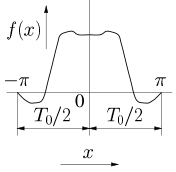
\includegraphics[width=3cm,trim=0 0 0 -5]{./bilder/gerade_funktion.png}&
        	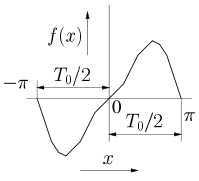
\includegraphics[width=3cm]{./bilder/ungerade_funktion.png}&
 			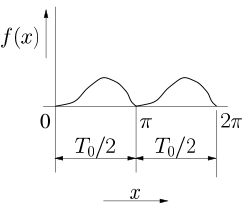
\includegraphics[width=3cm]{./bilder/halbperiode_1.png}&   
			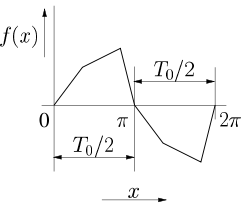
\includegraphics[width=3cm]{./bilder/halbperiode_2.png}\\
			\hline & & & \\			
   			$f(-t)=f(t)$ & $f(-t)=-f(t)$ & $f(t)=f(t+\pi)$ & $f(t)=-f(t+\pi)$\\
   			$b_k=0$ & $a_k=0$ & $a_{2k+1}=0$ & $a_{2k}=0$\\
   			$a_k = \frac{4}{T} \int\limits_0^{\frac{T}{2}} f(t) \cdot \cos(k \omega_1
   			t) dt$ &
   			$b_k =  \frac{4}{T} \int\limits_0^{\frac{T}{2}} f(t) \cdot
			\sin(k \omega_1 t) dt$ &
			$b_{2k+1}=0$ & $b_{2k}=0$\\
			\hline
      	\end{tabular}

	\subsection{Rechtecksignale}
	$$a_k=\frac{2}{T}\int\limits_{-t_1/2}^{t_1/2}A\cos\left(\frac{2\pi k}{T}t\right)dt=
	\left .\frac{2AT}{2\pi T k}\sin \left(\frac{2\pi k}{T}t\right)\right |_{-t_1/2}^{t_1/2}=
	\frac{2A}{\pi k}\sin\left(\frac{\pi t_1}{T}k\right)$$
	
	F"ur Verh"altnisse $\frac{T}{ggT(t_1,T)}=n\in\mathbb{N}$ verschwinden die
	$n.$ Harmonische und deren Vielfache.\\
	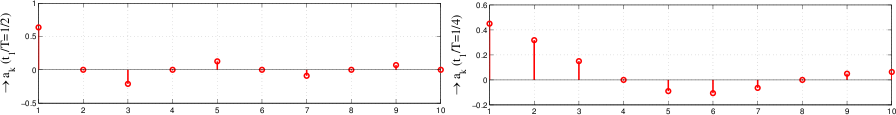
\includegraphics[width=19cm]{./bilder/fourierreihe-rechteck.png}
	
% Fourier-Integral / Fourier-Transformation
\section{Fourier-Transformation}
\begin{tabular}{|p{6cm} l|} \hline
	\textbf{Fouriertransformierte:} &
	$F(j\omega) = \int\limits_{-\infty}^{\infty} f(t)e^{-j\omega t}dt$ \\
	\textbf{Rücktransformierte:} &
	$f(t) = \frac{1}{2\pi}\int\limits_{-\infty}^{\infty}F(j\omega)e^{j\omega t}d\omega$ \\ \hline
\end{tabular} \\
\begin{tabular}{p{6cm} l}
Dies ergibt das \textbf{Korespondenzpaar:}	& $f(t) \laplace F(\omega)$ \\
											 & $F(t) \laplace 2\pi \cdot f(-\omega)$ \\
\end{tabular} \\
\begin{tabular}{p{6cm} l}
$F(\omega) = R(\omega) -jX(\omega)$ wobei &
$R(\omega) = \int\limits_{-\infty}^\infty f(t)\cdot \cos(\omega t)\,dt \quad \text{und} \quad X(\omega) =
\int\limits_{-\infty}^\infty f(t)\cdot \sin(\omega t)\,dt$ \\
 & $f(t)$ gerade: $X(\omega)$ verschwindet, f(t) ungerade: $R(\omega)$ verschwindet \\
\end{tabular} \\

Jede reelle $f(t)$ lässt sich aus Summe einer geraden und einer ungeraden Funktion beschreiben:\\
\begin{tabular}{lll}
$f(t) = f_e(t) + f_o(t)$ mit & $f_e(t) = \frac{1}{2}[f(t) + f(-t)]$ & $f_o(t) = \frac{1}{2}[f(t) - f(-t)]$ \\

Also: & $R(\omega) = 2 \int\limits_0^\infty f_e(t) \cos(\omega t)\,dt$ & $X(\omega) = 2 \int\limits_0^\infty
f_o(t) \sin(\omega t)\,dt$ \\

Und: & $f_e(t) = \frac{1}{\pi}\int\limits_0^\infty R(\omega)\cos(\omega t)\,d\omega$ & 
$f_o(t) = \frac{1}{\pi}\int\limits_0^\infty X(\omega)\sin(\omega t)\,d\omega$ \\
\end{tabular}

Bei \textbf{kausalen} Funktionen gilt:\\
$f_e(t) = f_o(t) = \frac{1}{2}f(t) \quad \quad \quad
f(t) = \frac{2}{\pi}\int\limits_0^\infty R(\omega) \cos(\omega t)\,dt = \frac{2}{\pi}\int\limits_0^\infty X(\omega)
\sin(\omega t)\,dt$

\begin{tabular}{|l|l|l|}
\hline
Spektraldichte / Spektraldarstellung	& $F(\omega)$ 		& KEINE absoluten Werte für Amplitude \& Phase \\
\hline
Amplitudendichte 						& $|F(\omega)| $		& f reell $\rightarrow$
$|F(\omega)|$ symetrisch zur Ordinatenachse
\\
\hline
Phasendichte							& $arg(F(\omega))$	& f reell $\rightarrow$ $arg(F(\omega))$ punktsymetrisch zum Ursprung \\
\hline
Kosinusamplitudendichte					& $R(\omega)$		& f reell $\rightarrow$ $R(\omega)$ gerade \\
\hline
Sinusamplitudendichte					& $X(\omega)$ 		& f reell $\rightarrow$ $X(\omega)$ ungerade \\
\hline
Dämpfung / Amplitudengang				& $A(\omega) = |H(\omega)|$ & $= \sqrt{H(\omega)\cdot \overline{H(\omega)}}$  \\
\hline
Phasenverschiebung						& $\Phi(\omega) = arg(H(\omega))$ & $= \arctan(\frac{Im(H(\omega))}{Re(H(\omega))})$ \\
\hline
\end{tabular}

\subsection{Symmetrie}
	Es gelten die gleichen Symmetrien wie bei der Fourierreihe.

\subsection{Hilbert-Transformation}
Das folgende Paar heisst \textit{Hilbert-Transformationspaar} und ermöglicht die Berechnung von Real- und Imaginärteil
einer Fouriertransformation auseinander. \\ 

\begin{tabular}{|l|} \hline
$\Re(\omega) = \frac{1}{\pi} \cdot \int\limits_{-\infty}^{\infty} \frac{\Im(u)}{\omega-u}du$ \\
$\Im(\omega) = -\frac{1}{\pi} \cdot \int\limits_{-\infty}^{\infty} \frac{\Re(u)}{\omega-u}du$ \\ \hline
\end{tabular} \\

Allgemein ist die Hilbert-Transformation $\mathcal{H}$ folgendermassen definiert: \\
$\mathcal{H}(f(t)) := \frac{1}{\pi} \cdot \int\limits_{-\infty}^{\infty} \frac{f(u)}{t-u}du$ \\

\subsection{Eigenschaften}
		\begin{tabular}{|p{8cm}|p{8cm}|}
        	\hline
        	Linearität & 
        	$\alpha\cdot f(t) + \beta\cdot g(t) \laplace \alpha\cdot F(j\omega) +
        	\beta\cdot G(j\omega)$\\
        	\hline
			Zeitumkehrung (Spiegelung an der Y-Achse)&
			$f(-t) \laplace F(-j\omega) = F^*(jw)$ \\
			\hline        	
  			"Ahnlichkeit / Zeitskalierung &
  			$f(\alpha t) \laplace \frac{1}{|\alpha|}F \left (j\frac{\omega}{\alpha} \right)
  			\quad\alpha \in\mathbb{R}\setminus \{0\}$\\
  			\hline
  			Verschiebung im	Zeitbereich &
  			$f(t\pm t_0) \laplace F(j\omega)e^{\pm j\omega t_0}$\\
  			\hline
			Verschiebung im Frequenzbereich &
			$f(t)e^{\pm j\omega_0 t} \laplace F(j(\omega\mp\omega_0))$\\
			\hline
			Ableitung im Zeitbereich &
			$\frac{\partial^n f(t)}{\partial t^n} \laplace (j\omega)^n F(j\omega)$\\
			\hline
			Integration im Zeitbereich &
			$\int\limits_{-\infty}^{t}f(\tau)d\tau \laplace
			\frac{F(j\omega)}{j\omega}+F(0)\pi\delta(\omega)$\\
			\hline				
			Ableitung im Frequenzbereich &
			$t^n f(t) \laplace j^n \frac{\partial F(j\omega)}{\partial \omega^n}$\\
			\hline		
			Faltung im Zeitbereich &
			$f(t) \ast g(t) = \int\limits_{-\infty}^{\infty} f(\tau)g(t-\tau)d\tau \laplace
			F(j\omega) \cdot G(j\omega)$\\
			\hline
			Faltung im Frequenzbereich &
			$f(t) \cdot g(t) \laplace \frac{1}{2\pi}F(j\omega) \ast G(j\omega)$\\
			\hline
			Vertauschungssatz (Dualität) &
			$f(t) \laplace F(j\omega)\nonumber$ \\
 			& $F(t) \laplace 2\pi \cdot f(-j\omega)$\\
 			\hline
 			Modulation &
 			$\cos(\alpha t) \cdot f(t)  \laplace  \frac{1}{2}\cdot
 			\left[F(j(\omega-\alpha)) + F(j(\omega+\alpha))\right ]$\\
 			& $\sin(\alpha t) \cdot f(t) \laplace \frac{1}{2j}\cdot \left[
 			F(j(\omega-\alpha)) - F(j(\omega+\alpha))\right ]$\\
 			\hline
        	Parseval's Theorem &
 			$\int\limits_{-\infty}^{\infty}f(t)g^{\ast}(t)dt = \frac{1}{2\pi}
  			\int\limits_{-\infty}^{\infty}F(j\omega)G^{\ast}(j\omega)d\omega$\\
  			\hline
  			Bessel's Theorem &
  			$\int\limits_{-\infty}^{\infty}|f(t)|^2 dt = \frac{1}{2\pi}
  			\int\limits_{-\infty}^{\infty}|F(j\omega)|^2 d\omega$\\
  			\hline 			
			Anfangswerte &
			$f(0)=\frac{1}{2\pi}\int\limits_{-\infty}^{\infty}F(j\omega)d\omega
			\hspace*{1cm} F(0)=\int\limits_{-\infty}^{\infty}f(t)dt$\\
			\hline
			$\infty$ lange Folge von $\delta$-Impulsen &
			$\sum_{n=-\infty}^{\infty} \delta(t-n\cdot t_0) \laplace
			\sum_{n=-\infty}^{\infty} \frac{2\pi}{t_0}\delta(\omega-n\cdot
			\frac{2\pi}{t_0})$\\
			\hline
        \end{tabular}
        
\subsection{Beispiele}
\begin{tabular}{l l}
Rechteckimpuls $r_T$ der Breite $2T$ & $r_T \laplace \frac{2 \cdot \sin(\omega T}{\omega}$ \\
Signum-Funktion & $\frac{1}{\pi \cdot t} \laplace -j \cdot sgn(\omega)$ \\
				& $sgn(t) \laplace \frac{2}{j\omega}$ \\
\end{tabular}


% LaPlace-Transformation

\section{Laplace-Transformation}
	$$\boxed{f(t) \; \laplace \; F(s)=\int\limits_0^\infty f(t)e^{-st}dt} \qquad \boxed{ s=\sigma+j\omega}$$\\
	\begin{tabular}{p{0.5cm}p{17.5cm}}
		$\bullet$ & Definitionsbereich nur für kausale Systeme $t\geq 0$\\
		%$\bullet$ & Integrierbar über das Intervall $(0,\infty)$\\
		$\bullet$ & Wachstum kleiner als der von einer Exponentialfunktion\\ 
		$\bullet$ & Gegen"uber $j\omega$ bei der Fourier-Transformation ist bei der
			Laplace-Transformation $s$ verallgemeinert zu $s=\sigma + j\omega$. Das
			bedeutet, dass die Fourier-Transformierte $F(j\omega)$ durch die
			Laplace-Transformation $F(s)$ ausgedr\"uckt werden kann. \\
		$\bullet$ & mit 
		$\begin{cases} 
		\sigma = 0 & \rightarrow \text{Amplitude bleibt konstant} \\ 
		\sigma > 0 & \rightarrow \text{explodiert die Amplitude f\"ur } 0 < t \rightarrow \infty \\
		\sigma < 0 & \rightarrow \text{klingt die Amplidute für } 0 < t \rightarrow \infty \text{ auf $0$ ab} \
		 \end{cases} $ \\   
	\end{tabular}
	
 	\subsection{Eigenschaften der Laplace-Transformation}
  		\renewcommand{\arraystretch}{2}
		\begin{tabular}{|ll|}
	        \hline
	        	Linearität & 
	 			$\alpha\cdot f(t) + \beta\cdot g(t) \; \laplace \; \alpha\cdot F(s) + \beta\cdot
	 			G(s)$ \\
			\hline
	 			"Ahnlichkeit / Streckung im Zeitbereich &
	 			$f(\alpha t) \; \laplace \; \frac{1}{\alpha}F \left (\frac{s}{\alpha} \right ) \quad 0 <\alpha, \alpha \in\mathbb{R}$ \\
	 		\hline
	 		\hline
	 			Faltung im Zeitbereich &
	 			$f(t) \ast g(t) = \int\limits_{0}^{t} f(\tau)g(t-\tau)d\tau \; \laplace \; F(s)
	 			\cdot G(s)$\\
	 		\hline
	 			Faltung im Frequenzbereich &
	 			$f(t) \cdot g(t) \; \laplace \; \frac{1}{2\pi j}\int\limits_{c-j\infty}^{c+j\infty}
	 			F(\xi) G(s-\xi)d\xi$ \\
	 		\hline
	 		\hline
	 			1te Ableitung im Zeitbereich &
	 			$\frac{\partial f(t)}{\partial t} \; \laplace \; sF(s)
	 			-f(0^+)$ \\
	 		\hline
	 			2te Ableitung im Zeitbereich &
	 			$\frac{\partial f(t)}{\partial t} \; \laplace \; s^2F(s)
	 			-sf(0^+) -f'(0^+)$ \\
	 		\hline
	 			nte Ableitung im Zeitbereich &
	 			$\frac{\partial^n f(t)}{\partial t^n} \; \laplace \; s^nF(s)
	 			-s^{n-1}f(0^+)-s^{n-2}\frac{\partial f(0^+)}{\partial t}-\ldots
	 			-s^0\frac{\partial^{n-1} f(0^+)}{\partial t^{n-1}}$ \\
	 		\hline
	 			Ableitung im Frequenzbereich &
		 		$(-t)^n f(t) \; \laplace \;  \frac{\partial^n F(s)}{\partial s^n}$ \\
	 		\hline
	 		\hline
	 			Verschiebung im Zeitbereich nach rechts &
	 			$\sigma(t-a)f(t - a) \; \laplace \; F(s)*e^{-as}$ \\
	 		\hline
				Verschiebung im Zeitbereich nach links &
				$\sigma(t-a)f(t + a) \; \laplace \; e^{as} \cdot [F(s) - \int\limits_0^{a} f(t) \cdot e^{-st} dt]$\\
			\hline
	 			Verschiebung im Frequenzbereich (Dämpfungssatz) &
	 			$f(t)e^{\pm\alpha t} \; \laplace \; F(s\mp\alpha)$ \\
	 		\hline
	 		\hline
	 			Integration im Originalbereich (Sprungantwort)&
	 			$\int\limits_0^t f(u)du \; \laplace \; \frac{1}{s}\cdot F(s)$ \\
	 		\hline
	 			Multiplikation mit $t$ &
	 			$t\cdot f(t)  \; \laplace \; \frac{-\partial F(s)}{\partial s}$ \\
 			\hline
 			\hline
	 			Anfangswert &
	 			$\lim_{t\rightarrow 0^+} f(t) = \lim_{s\rightarrow \infty} sF(s),\text{~wenn
	 			}  \lim_{t\rightarrow 0} f(t)\text{~existiert}.$ \\
 			\hline
	 			Endwert &
	 			$\lim_{t\rightarrow \infty} f(t) = \lim_{s\rightarrow 0} sF(s),\text{~wenn
	 			}  \lim_{t\rightarrow \infty} f(t)\text{~existiert}.$ \\
	 		\hline
       	\end{tabular}
		\renewcommand{\arraystretch}{\arraystretchOriginal}
	
	\subsection{Laplace-Tabelle}
	\renewcommand{\arraystretch}{2}
	\hrule
	\begin{minipage}{9cm}
		\begin{center}
			\begin{tabular}{p{4cm}p{0.75cm}p{3cm}}
				$\sigma \left( t \right)$ & $\; \laplace \;$ & $\dfrac{1}{s}$ \\
				
				$\sigma \left( t \right) \cdot t$ & $\; \laplace \;$ & $\dfrac{1}{s^2}$\\
				
				$\sigma \left( t \right) \cdot t^2$ & $\; \laplace \;$ & $\dfrac{2}{s^3}$\\
				
				$\sigma \left( t \right) \cdot t^n$ & $\; \laplace \;$ & $\dfrac{n!}{s^{n+1}}$\\
				
				$\sigma \left( t \right) \cdot e^{\alpha t}$ & $\; \laplace \;$ &
				$\dfrac{1}{s-\alpha}$\\
				
				$\sigma \left( t \right) \cdot t \cdot e^{\alpha t}$ & $\; \laplace \;$ & $\dfrac{1}{( s - \alpha )^2}$\\
				
				$\sigma \left( t \right)\cdot t^2 \cdot e^{\alpha t}$ &
				$\; \laplace \;$ & $\dfrac{2}{{( s - \alpha )}^3}$\\
				
				$\sigma \left( t \right)\cdot t^n \cdot e^{ \alpha t}$ &
				$\; \laplace \;$ & $\dfrac{n!}{(s-\alpha)^{n+1}}$\\
				
				$\sigma \left( t \right)\cdot \dfrac { 1 - e ^ { - \alpha t } } { \alpha }$ & $\; \laplace \;$ & $\dfrac { 1 } { s ( s + \alpha ) }$\\
				
				$\sigma \left( t \right)\cdot \dfrac {e ^ { - \alpha t }+\alpha t -1 } { \alpha^2 }$ & $\; \laplace \;$ & $\dfrac { 1 } { s^2 ( s + \alpha ) }$\\
				
				$\sigma \left( t \right)\cdot \dfrac {1- e ^ { - \alpha t } - \alpha t e ^ {- \alpha t }}{ \alpha ^2 }$ & $\; \laplace \;$ & $\dfrac { 1 } { s ( s + \alpha )^2 }$\\
					
			\end{tabular}
		\end{center}
	\end{minipage}
\vline
\begin{minipage}{9cm}
\begin{center}
	\begin{tabular}{p{5cm}p{0.75cm}p{3cm}}
	
		$\delta \left( t \right)$ & $\; \laplace \;$ & $1\left( s \right)$ \\
		
		$\delta \left( t - \alpha \right)$ & $\; \laplace \;$ & $e^{- \alpha s}$\\
		
		$\sigma\left( t - \alpha \right)$ & $\; \laplace \;$ & $ \dfrac{1}{s} \cdot e^{- \alpha s}$\\
		
		$\sigma \left( t \right) \cdot \sin \left(\omega t \right)$ & $\; \laplace \;$ &
		$\dfrac{\omega}{s^2 + {\omega^2}}$\\
		
		$\sigma \left( t \right) \cdot \cos \left( \omega t \right)$ & $\; \laplace \;$ &
		$\dfrac{s}{ s^2 + \omega^2}$\\
		
		$\sigma \left( t \right) \cdot  e^{ \alpha t} \cdot \sin \left(\omega t \right)$ & $\; \laplace \;$ 
		& 	$\dfrac{\omega}{(s-a)^2 + {\omega^2}}$\\
		$\sigma \left( t \right) \cdot e^{ \alpha t} \cdot \cos \left( \omega t \right) $ & $\; \laplace \;$ &
		$\dfrac{s-a}{(s-a)^2 + \omega^2}$\\
		
		$\sigma \left( t \right)\cdot t \cdot \dfrac{\sin \left( \alpha t \right)} { 2 \alpha }$ & $\; \laplace \;$ & $\dfrac{s}{ \left(s^ {2}+ \alpha ^{2} \right)^{2}}$ \\
		
		$\sigma \left( t \right)\cdot \dfrac { e ^ { - \alpha t } - e ^ { - \beta t } } { \beta - \alpha }$ & $\; \laplace \;$ & $\dfrac { 1 } { ( s + \alpha ) ( s + \beta ) }$\\
		
		$\sigma \left( t \right)\cdot \dfrac {(\alpha - \beta) +\beta e ^ { - \alpha t } - \alpha e ^ { - \beta t } } { \alpha \beta (\alpha - \beta) }$ & $\; \laplace \;$ & $\dfrac { 1 } {s ( s + \alpha ) ( s + \beta ) }$\\
		
		$\sigma \left( t \right)\cdot \dfrac { e ^ { - \beta t } ( \alpha \cos ( \alpha t ) - \beta \sin ( \alpha t ) ) } { \alpha }$& $\; \laplace \;$ & $\dfrac { s } { ( s + \beta ) ^ { 2 } + \alpha ^ { 2 } }$\\
		
		 
		
		
	\end{tabular}
\end{center}
\end{minipage}


\newpage
\renewcommand{\arraystretch}{\arraystretchOriginal}		
	\subsection{Rücktransformation}
		\subsubsection{Vorgehen}
				1. Kürzen oder vereinfachen \\
				2. Partialbruchzerlegung falls nötig \\
				3. Rücktransformation mittels Laplace-Tabelle \\
				4. $h(t)\hspace{0.2cm}\underline{nicht} < 0$ \\
			
		\subsubsection{Residuensatz}
			Beispiel:\\
			$F(s) = \frac{1}{(s+\alpha)(s+\beta)}, \qquad (0 < \alpha,\beta \in \mathbf{R}, \alpha \neq \beta)$\\
			$f(t) = \frac{1}{2\pi j} \int\limits_{-j\infty}^{j\infty} F(s)e^{st} ds = \sum\limits_{i=1}^k Res(F(s_k)e^{s_kt})$\\
			$=\lim_{s \to -\alpha} ((s+\alpha)F(s)e^{st}) + \lim_{s \to -\beta}((s+\beta)F(s)e^{st})$\\
			$=\frac{e^{-\alpha t}}{\beta - \alpha} + \frac{e^{-\beta t}}{\alpha - \beta} = \frac{e^{-\alpha t}-e^{-\beta t}}{\beta - \alpha}$
			
			
	\subsection{Lösung linearer Differentialgleichungen}
		\begin{minipage}{11.5cm}
			\renewcommand{\arraystretch}{2}
			\begin{tabular}{| l | l |}
				\hline
					Übertragungsfunktion & $G(s) = \frac{1}{p(s)}$\\
					& $g(t) \; \laplace \; G(s)$ \\
				\hline
					Frequenzgang & $G(j\omega) = H(\omega)$ \\
				\hline
					Impulsantwort & $y_{\delta}(t) = g(t) = y_{\sigma}'(t) \; \laplace \; G(s) = \frac{1}{p(s)}=Y_{\delta}(s)$\\
				\hline
					Sprungwantwort & $y_{\sigma}(t)=\int\limits_0^t g(u) du \; \laplace \; \frac{G(s)}{s} = \frac{1}{s \cdot p(s)} = Y_{\sigma}(s)$\\
				\hline
					Eigenschwingung & $\frac{h(s)}{p(s)}$ \\
				\hline
					äussere Erregung & $\frac{F(s)}{p(s)}$ \\
				\hline
					stationärer Zustand & = ungedämpfte Eigenschwingung\\
				\hline
			\end{tabular}
			\renewcommand{\arraystretch}{\arraystretchOriginal}\\
		\end{minipage}
		\begin{minipage}{8cm}
					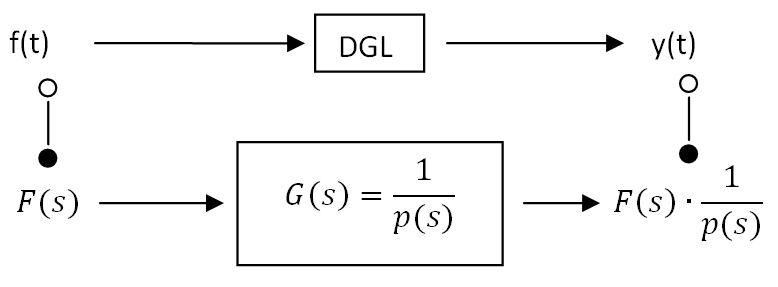
\includegraphics[width=8cm]{./bilder/diffgleichungen2.png} \\
		\end{minipage}
		
		
		\begin{minipage}[l]{16cm}
				\textbf{Beispiel:} $y'' + 8y' + 25y = \sigma{t} \cdot \sin(2t)$ mit $y(0) = 2, y'(0) = -1$\\
				
				$\sin(2t) \; \laplace \; \frac{2}{s^2+4}$ \\ $Y(s)(s^2+8s+25) = 2s+15+\frac{2}{s^2+4}$
				$\Leftrightarrow Y(s) = \frac{2s+15}{s^2+8s+25}+\frac{2}{(s^2+4)(s^2+8s+25)}=
				\underbrace{\frac{2s+15}{s^2+8s+25}}_\text{Eigenschwinung durch Anfangszustand} +
				\underbrace{\frac{As + B}{s^2+4}}_\text{stationärer Zustand} +
				\underbrace{\frac{Cs + D}{s^2+8s+25}}_\text{Eigenschwinung durch Einschalten}$
		\end{minipage}
		\subsubsection{Eigenschwingungen}
			Aus der Eigenschwingung können die Nullstellen des charakteristischen Polynom $p(s)$ 
			direkt abgelesen werden. \\
			\textbf{Beispiel:} \\
			$y(t) = \frac{1}{2} e^{-t} \sin(3t) - \frac{2}{3} e^{-2t} \cos(2t) = 
			\underbrace{\frac{1}{2} e^{\textcolor{red}{-t}} \frac{1}{2j}(e^{\textcolor{red}{3j}t}
			-e^{\textcolor{red}{-3j}t})}_{NS = EW = \textcolor{red}{-1 \pm 3j}} - 
			\underbrace{\frac{2}{3} e^{\textcolor{red}{-2}t} \frac{1}{2}(e^{\textcolor{red}{2j}t}
			+e^{\textcolor{red}{-2j}t})}_{NS = EW = \textcolor{red}{-2 \pm 2j}}$ \\\\
			Damit ist das char. Polynom $p(s) = (s-NS_1)(s-NS_2)\ldots(s-NS_n)$ \\
			Bei mehreren gemessenen Eigenschwingungen werden die char. Polynome multipliziert. \\
			Der stationäre Zustand ist $\lim\limits_{t\rightarrow\infty}y(t) = \frac{1}{p(0)}$ *(Endwertsatz) \\
				
		
	\subsection{Eigenschwingung}
		\begin{minipage}{12cm}
			Spezielle Anfangswerte bei einem System ohne äussere Einflüsse:\\
			$y(0) = 0, y'(0) = 0, \dots , y^{(n-2)} = 0, y^{(n-1)} = 1$\\
			in diesem Fall wird $h(s) = 1$\\
		\end{minipage}
		\begin{minipage}{6cm}
			\begin{math}
				\begin{aligned}
					y(t) \; &\laplace \; Y(s)\\
					y'(t) \; &\laplace \; sY(s) - y_0\\
					y''(t)\; &\laplace \; s^2Y(s) - sy_0 - y'_0\\ 
					y'''(t)\; &\laplace \; s^3Y(s) - s^2y_0 - sy'_0 - y''_0\\ 
					\vdots&\\
					y^{(n)} \; &\laplace \; 
					\underbrace{s^nY(s)}_{Y(s) \cdot p(s)}
					\underbrace{-s^{n-1}y_0 - \dots - y^{(n-1)}}_{h(s)}
				\end{aligned}
			\end{math}
		\end{minipage}

% Diverses
\newpage
\section{Diverses}
\subsection{Partialbruchzerlegung}
	\[f(x)=\frac{x^2+20x+149}{x^3+4x^2-11x-30} \Rightarrow \; \begin{array}{l}\text{Nenner faktorisieren mit}\\
	\text{Hornerschema, Binom, etc.}\end{array} \Rightarrow
	x^{3}+4x^{2}-11x-30=(x+2)(x^{2}+2x-15)=(x+2)(x+5)(x-3)\] Ansatz:
	\[f(x)=\frac{x^2+20x+149}{x^3+4x^2-11x-30}=\frac{A}{x-3} + \frac{B}{x+2} + \frac{C}{x+5}=
	\frac{A(x+2)(x+5)+B(x-3)(x+5)+C(x-3)(x+2)}{(x-3)(x+2)(x+5)}\]
	Gleichungssystem aufstellen mit beliebigen $x_i$-Werten (am Besten Polstellen oder 0,1,-1 wählen):
	\[\begin{array}{l}x_1=3:\;-9+60+149=A\cdot5\cdot8\;\;\;\Rightarrow A=5\\
	x_2=-2:\;-4-40+149=B(-5)\cdot3\; \Rightarrow B=-7\\
	x_3=-5:\;-25-100+149=C(-8)(-3) \Rightarrow C=1 \end{array} \Rightarrow
	f(x)=\frac{5}{x-3}-\frac{7}{x+2}+\frac{1}{x+5}\] weitere Ansätze für andere
	Typen von Termen: \[f(x)=\frac{5x^2-37x+54}{x^3-6x^2+9x}=\frac{A}{x}+\frac{B}{x-3}+\frac{C}{(x-3)^2}=\frac{A(x-3)^2+Bx(x-3)+Cx}{x(x-3)^2}\]
	\[f(x)=\frac{1,5x}{x^3-6x^2+12x-8}=\frac{A}{x-2}+\frac{B}{(x-2)^2}+\frac{C}{(x-2)^3}=\frac{A(x-2)^2+B(x-2)+C}{(x-2)^3}\]
	\[f(x)=\frac{x^2-1}{x^3+2x^2-2x-12}=\frac{A}{x-2}+\frac{Bx+C}{x^2+4x+6}=\frac{A(x^2+4x+6)+(Bx+C)(x-2)}{(x-2)(x^2+4x+6)}\]

	Variante mit Koeffizientenvergleich: \\
	\[F(s) = \frac{1}{s(s^2+6s+13)} = \frac{A}{s} + \frac{Bs+C}{s^2+6s+13}\]
	\[1 = A(s^2+6s+13) + s(Bs+C) \]
	\[1 = s^2(A+B) + s(C+6A) + 13A \]
	\[\Rightarrow 1 = 13A; (A+B)=0; (C+6A)=0 \]
	\[\Rightarrow A=\frac{1}{13}; B=-\frac{1}{13}; C=-\frac{6}{13}\]

			
\subsection{Hornerschema}
	\begin{minipage}[t]{9cm}
		- Pfeile $\Rightarrow$ Multiplikation\\
		- Zahlen pro Spalte werden addiert\\
		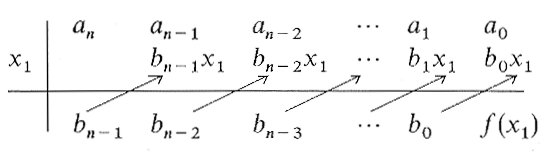
\includegraphics[width=6cm]{./bilder/hornerschema_1.png}\\
		$x_1 \Rightarrow$ Nullstelle (muss erraten werden!!)\\
		oberste Zeile = zu zerlegendes Polynom			
	\end{minipage}
	\begin{minipage}[t]{9cm}
		\textbf{Beispiel:}\\
		$f(x) = x^3-67x-126$\\
		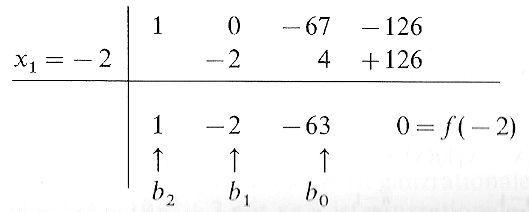
\includegraphics[width=6cm]{./bilder/hornerschema_2.png}\\
		$\Rightarrow f(x) = (x-x_1)(b_2x^2 + b_1x + b_0) = (x+2)(x^2-2x-63)$	
	\end{minipage}

\newpage

\subsection{Schrittfunktion - unit step}
	\begin{minipage}{10cm}
		$u(t) = \sigma(t) =	\begin{cases}
		  		 0 & \text{für } t < 0 \\
		  		 \frac{1}{2} \text{(praxis)}  \text{ oder undef. (math.)} & \text{für } t = 0 \\
		  		 1 & \text{für } t > 0
		  	\end{cases}
		$
		$\sigma(t) \laplace \frac{1}{j\omega} + \pi\delta(\omega) = \Sigma(\omega)$
	\end{minipage}
	\begin{minipage}{8cm}
		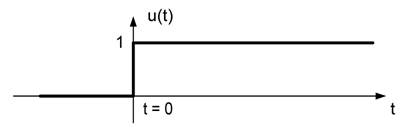
\includegraphics[width=6cm]{./bilder/unitstep.png}
	\end{minipage}

\subsection{Impulsfunktion - dirac delta function}
	\begin{minipage}{10cm}
		\begin{tabular}{l l}
		Definition & $\delta (t)=\begin{cases} 0 & t\ne 0\\\infty & t=0\end{cases}$ \\
				   & $\int\limits_{-\infty}^\infty \delta(t) \, \mathrm dt = 1 $ \\
		Zusammenhang mit der $\sigma$-Funktion & $\frac{d\sigma(t)}{dt}=\delta(t)$ \\
		Abtastung & $\int\limits_{-\infty}^{\infty} \delta(t-t_0)f(t)dt=f(t_0)$ \\
		Transformierte & $\delta(t) \laplace 1(\omega)$ \\
						& $1(t) \laplace 2\pi \cdot \delta(\omega)$ \\
		Faltung & $f(t) \ast \delta(t) = f(t)$ \\
		Ableitung & $\int\limits_{-\infty}^{\infty} \delta^{(k)}(t) \cdot f(t) dt = (-1)^k \cdot f^{(k)}(0)$ \\
		\end{tabular}
	\end{minipage}
	\begin{minipage}{8cm}
		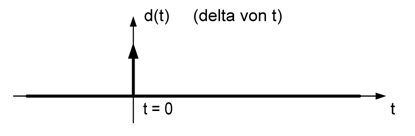
\includegraphics[width=6cm]{./bilder/diracimpulse.png}
	\end{minipage}

% Riisä Tricks
\section{Riisä Tricks und Merksätze}
\begin{itemize}
  \item $H(s)$ = UTF = Laplace-Transformierte der Impulsantwort ($y_\delta(t)$)
  \item $H(j \omega)$ = Frequenzgang = UTF auf imaginärer Achse
  \item $y_\sigma(t) = \int\limits_0^t y_\delta(u)du$
  \item $\left| \frac{ja + b}{a^2 + b^2} \right| = \sqrt{\frac{1}{a^2 + b^2}}$
  \item Dirac-Funktion: $s(t)\delta(t-t_0) = s(t_0)\delta(t-t_0)$
  \item Antwort eines LTI-Systems auf eine harmonisches Schwingung mit Frequenz $\omega \Rightarrow$ harmonische
  Schwingung mit gleicher Frequenz aber anderer Amplitude und Phase ($\mathcal{L}\{e^{j \omega t}\} = H(\omega) \cdot
  e^{j \omega t}$)
  \item $H(\omega)$ = komplexwertige Funktion der Frequenz $\omega$, die für jede Frequenz $\omega$ die
  Änderung von Amplitude und Phase durch das System speichert = Frequenzgang = Antwort auf harmonische Schwingung
  beliebiger Frequenz
\end{itemize}

\newpage

% Wichtige Formeln
\section{Idiotenseite}
%\subsection{Diverses}
\begin{tabbing}
	xxxxxxxxxxxxxxxxxxxxxxxxxxxx \= xxxxxxxxxxxxxxxxxxxxxxxxxxxxxx \= \kill
 	$f'(z) = \lim \limits_{\Delta z \rightarrow 0} \frac{f(z + \Delta z) -
	f(z)}{\Delta z}$ \> $(a + b)^n = \sum_{k=0}^{n} \binom n k a^{n-k} \cdot b^k$ \>
	$(a \pm b)^3 =a^3 \pm  3 a^{2} b + 3 a b^2 \pm b^3 $\\ \\
	$x_{1,2} = \dfrac{-b \pm \sqrt{b^2 - 4ac}}{2a}$ \> $\binom n k = \dfrac{n!}{k!
	\cdot (n-k)!}$ \> $(a \pm b)^4 =a^4 \pm  4 a^{3} b + 6a^2b^2 \pm 4 a b^3 +
	b^4$\\
\end{tabbing}
%\subsection{Reihenentwicklungen}
\begin{tabular}{llll}
\textbf{Geometrische Reihe}
	& $\sum\limits_{n=0}^{\infty} x^n$ 
	& $= \dfrac{1}{1-x}$
	& $|x| < 1$ \\
	
	& $\sum\limits_{k=0}^{\infty} k \, x^k$ & $= x \sum\limits_{k=1}^{\infty} k \,
	x^{k-1} = \dfrac{x}{(1-x)^2} $ 
	& $x \neq 1$ \\
\textbf{Binominalreihe} 
	& $\sum\limits_{n=0}^\infty \binom{\alpha}{n} x^n $ &$= (1+x)^\alpha$
	& $x \in (-1,1)$ \\
\textbf{E-Funktion}
	& $\sum\limits_{k = 0}^{\infty} \dfrac{x^k}{k!}$ &$ = e^x$
	& 
\end{tabular}

\newpage

% Integraltabelle
\section{Integralrechnung}
Partielle Integration: $\int u(x) v'(x) dx = u(x)v(x) - \int u'(x) v(x) dx$

\subsection{Einige wichtige Integrale}
  	\renewcommand{\arraystretch}{2}
	\begin{tabular}{|l|l|}
    	\hline
    	$\int \sin(x)dx=-\cos(x)$ & $\int \sin(a+bx)dx=-\frac1b \cos(a+bx)$\\
    	\hline
	  	$\int \sin^2(x)dx=-\frac14 \sin(2x)+\frac x2$ 
    	& $\int
    	e^{ax+c}\sin(bx+d)dx=\frac{e^{ax+c}}{a^2+b^2}(a\sin(bx+d)-b\cos(bx+d))$\\
    	\hline
    	$\int \cos(x)dx=\sin(x)$ & $\int \cos(a+bx)dx=\frac1b \sin(a+bx)$\\
    	\hline
	  	$\int \cos^2(x)dx=\frac14 \sin(2x)+\frac x2$ 
    	& $\int
    	e^{ax+c}\cos(bx+d)dx=\frac{e^{ax+c}}{a^2+b^2}(a\cos(bx+d)+b\sin(bx+d))$\\
    	\hline
    	$\int e^x dx=e^x$ & $\int e^{ax}dx=\frac1a e^{ax}$\\
    	\hline
    	$\int xe^{ax}dx=\frac{1}{a^2} e^{ax}(ax-1)$ & $\int x^2 e^{ax} dx =
    	e^{ax}\left( \frac{x^2}{a} - \frac{2x}{a^2} + \frac{2}{a^3}\right)$ \\
    	\hline
    	$\int x^n e^{ax} dx = \frac{1}{a} x^n e^{ax} - \frac{n}{a} \int x^{n-1}
    	e^{ax} dx$ & \\
    	\hline
    \end{tabular}

\section{Differentialrechnung}
\subsection{Einige wichtige Differentiale}
\begin{multicols}{2}
	\begin{tabular}{|l|l||l|l|}
    	\hline
    	\textbf{Funktion} & \textbf{Ableitung} & \textbf{Funktion} &
    	\textbf{Ableitung}\\
    	\hline
    	\hline
    	$C \text{ (Konstante)}$ & $0$ & $x$ & $1$\\
    	\hline
    	$x^n$ & $nx^{n-1}$ & $\frac1x$ & $-\frac{1}{x^2}$\\
    	\hline
    	$\sqrt{x}$ & $\frac{1}{2\sqrt{x}}$ & $e^x$ & $e^x$\\
    	\hline
    	$e^{bx}$ & $be^{bx}$ & $a^x$ & $a^x \ln(a)$\\
    	\hline
    	$\ln(x)$ & $\frac1x$ & $\sin(x)$ & $\cos(x)$\\
    	\hline
    	$\cos(x)$ & $-\sin(x)$ & $\ln[f(x)]$ & $\frac{f^{'}(x)}{f(x)}$\\
    	\hline	
    \end{tabular}
\columnbreak  	
\subsection{Aufgabenbeispiel}
$f(t) =\sum_{k=0}^{\infty}\delta (t-k\pi) \cdot cos(t)$ \\
$ = \sum_{k=0}^{\infty} = \delta (t-k\pi) \cdot cos(\pi t)  \\
\; \laplace \; 
F(s) = \sum_{k=0}^{\infty} (-1)^k(e^{-k\pi s}) \\
= \sum_{k=0}^{\infty} (-1)^k(e^{-\pi s})^k$ 
\\ \\
Die Summenformel der geometrischen Reihe liefert: \\
$F(s) = \dfrac{e^{-\pi s}}{1 +e^{-\pi s}}$ \\

\end{multicols}
\renewcommand{\arraystretch}{\arraystretchOriginal} 
\newpage


\end{document}